






% =========----------	[ Space left here for distraction free mode] ----------==========%










\section{Analysis Overview}

	All test data was recorded using a Google Form and collated into a large document upon finishing the testing period. All data was then imported into MATLAB for analysis. Table~\ref{image:results_sum} shows the average spatial attribute results for each microphone across each spatial attribute. The highest scores are highlighted in green. The directional OCT microphone array from microphone position and viewing position B scored highest for 'Locatedness' and scored the highest along with the Hamasaki Cube, a diffuse-field microphone array located at position C for 'Sense of Space'. The Hamasaki Cube when viewing from position A scored the highest for 'Externalisation' and 'Envelopment' which results in the highest over all spatial attribute average score. A break down of timbral attribute scores is covered in section~\ref{ana4}\\


	The following six sections will be used to further break down and analyse the data: \\

	\begin{tabular}{r p{5.5cm}}
		Analysis 1: & Does viewing position affect Spatial Attribute rating? \\
		Analysis 2: & Does the choice of microphone array affect Spatial Attribute score? \\
		Analysis 3: & What is the effect of using Directional or Diffuse-Field Arrays? \\ 
		Analysis 4: & Does perception of timbre change with difference viewing positions? \\
		Analysis 5: & Is there a correlation between spatial attribute score and selected timral attributes? \\
		Analysis 6: & Is there a correlation between the enjoyment rating and spatial audio attributes?
	\end{tabular}
	
	\begin{table}
	\begin{center}
		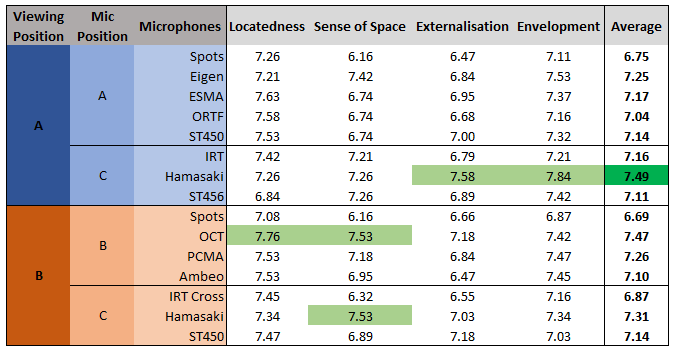
\includegraphics[width=0.45\textwidth]{images/graphs/results_sum_graph_V3.PNG}
		\caption{Table containing the average spatial attribute scores for all microphone with on over all average spatial attribute score. Highest scoring microphones are highlighted in green.}
		\label{image:results_sum} 
	\end{center}
	\end{table}	

	This will be followed by an summary section with conclusions draw from each analysis section.

	






% =========----------	[ Space left here for distraction free mode] ----------==========%









\subsection{Analysis 1: Does viewing position effect spatial attribute scores?}
	\label{ana1}

		% Ana1 Intro
		To assess the potential effect of viewing position on spatial attribute score, data was grouped into 8 sections: An average score for each spatial audio attribute (4 groups) each split into the average score for viewing position A and B (8 groups) illustrated in figure \ref{image:AvsB}. \\

		\begin{figure}
			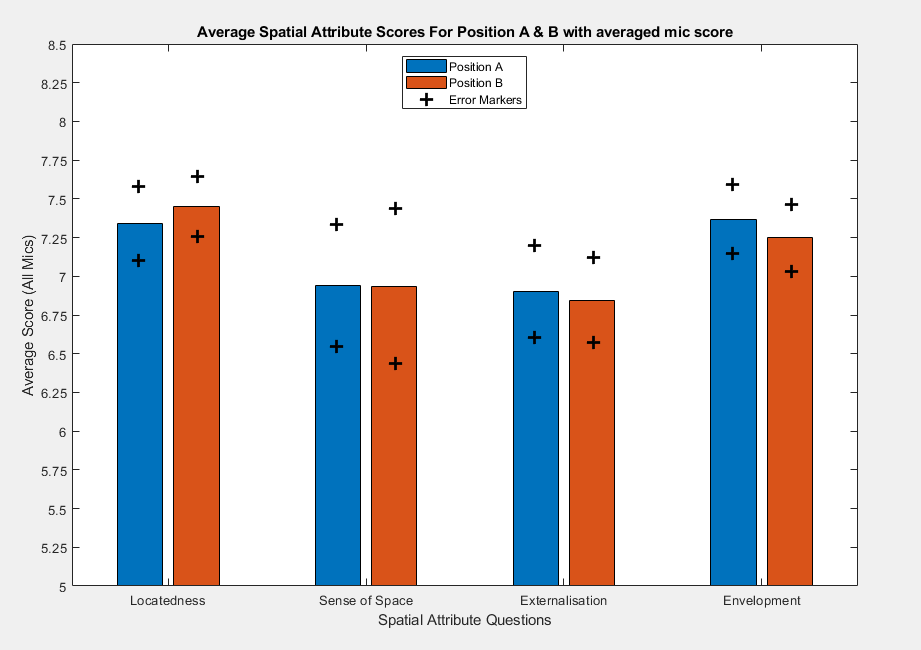
\includegraphics[width=0.5\textwidth]{images/plots/AvB_Bar_error.PNG}
			\caption{Bar chart showing average spatial attribute score for each spatial attribute at viewing position A and B}
			\label{image:AvsB} 
		\end{figure}

		It can be seen that the average spatial attribute score for viewing position A and B for each spatial attribute are close with the difference in overall mean score being 0.02. Running a Two-Sample T-Test between each of the four spatial attribute groups (e.g A vs B for locatedness etc) indicates no statistical significance. Running the same test for the averaged combined spatial attribute score (average of all four spatial attribute scores) also indicates no statistical significant between viewing position. This is made clear in figure \ref{image:AvsB_dist} illustrating the overall similarity in the distribution of scores for viewing position A and B. \\
		
		% NOTE: Should I display the distributiong as 'normal' or 'kernel'?
		\begin{figure}
			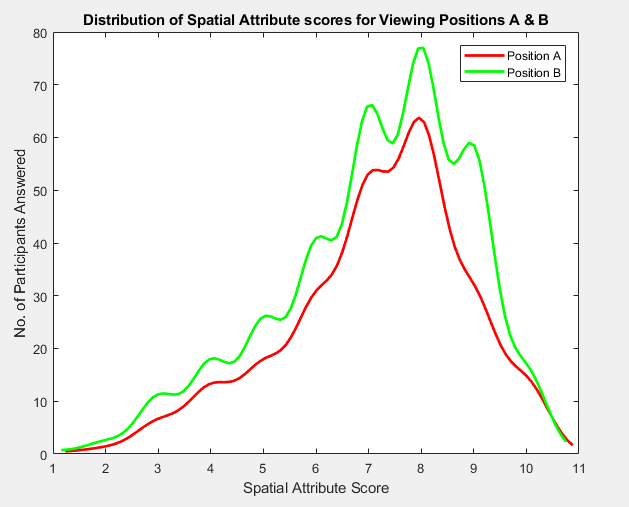
\includegraphics[width=0.5\textwidth]{images/stats/AvsB_sa_stack_all.PNG}
			\caption{Histogram showing the distribution of spatial attribute scores for viewing position A and B. This indicates that viewing position has little effect on spatial qualities in a VR environment.}
			\label{image:AvsB_dist} 
		\end{figure}

		\textbf{Conclusion}\\

		The bar chart indicates that the average spatial attribute scores are extremely close with an overall average for both being 7.1. The Two-Sample T-Test indicates that the probability of these results recurring is not unlikely ($p > \alpha (0.05)$) and therefore the results shown are not statistically significant.


	






% =========----------	[ Space left here for distraction free mode] ----------==========%









\subsection{Analysis 2: Does the choice of microphone array effect Spatial Attribute score?}
	\label{ana2}

		Breaking down the data showing in figure~\ref{image:AvsB}, figure~\ref{image:sa_allmics} shows the average spatial attribute score across all used microphone configurations. The Anderson-Darling test was used to determine that not all of the sample data (participants scores per microphone) is normally distributed. Due to non-normally distributed data the Kurskal-Wallis (K-W) ANOVA was used to determine whether any of the samples were significantly different. \\

		All groups returned a p-value greater than 0.05 other than 'Sense of Space' which returned $p = 0.0227 $. As determined in section~\ref{ana1} there is no statistical significant difference between the data from viewing positions A and B. Therefore the data was separated according to their viewing positions and another K-W test was conducted on each group. This indicated a significant difference within the group of data from viewing position B, returning $ p = 0.0035 $.

		Using MATLABs \textit{multcompare} function, a post-hoc test was conducted to determine that the sample data for two microphone arrays, OCT and Hamasaki Cube were significantly different to the sample data for the spot microphones, circled in red and blue respectively in figure~\ref{image:sa_allmics}. \\

		% NOTE: SHOULD THIS PARAGRAPH BE HERE AS IT HAS BEEN SHOWN THAT THERE IS NO STATISTICAL SIGNIFICANCE IN THE DIFFERENCES IN SCORE?
		Though little statistical significance was found between the difference microphone arrays, by analysing figure~\ref{image:sa_allmics} we can determine which microphones are overall the best choice with regards to this listening test. The two microphone arrays that showed statistical significance, the OCT and Hamasaki Cube also happen to consistently be among the top scoring microphone arrays across all spatial attributes.

		\textbf{Conclusion} \\

		For most spatial attributes, differences in mic choice is not statistically significant. However when it comes to sense of space, mixing in the microphone arrays with either the OCT or Hamasaki cube makes a significant difference relative to a pure spot mic mix. 

		\begin{figure}
			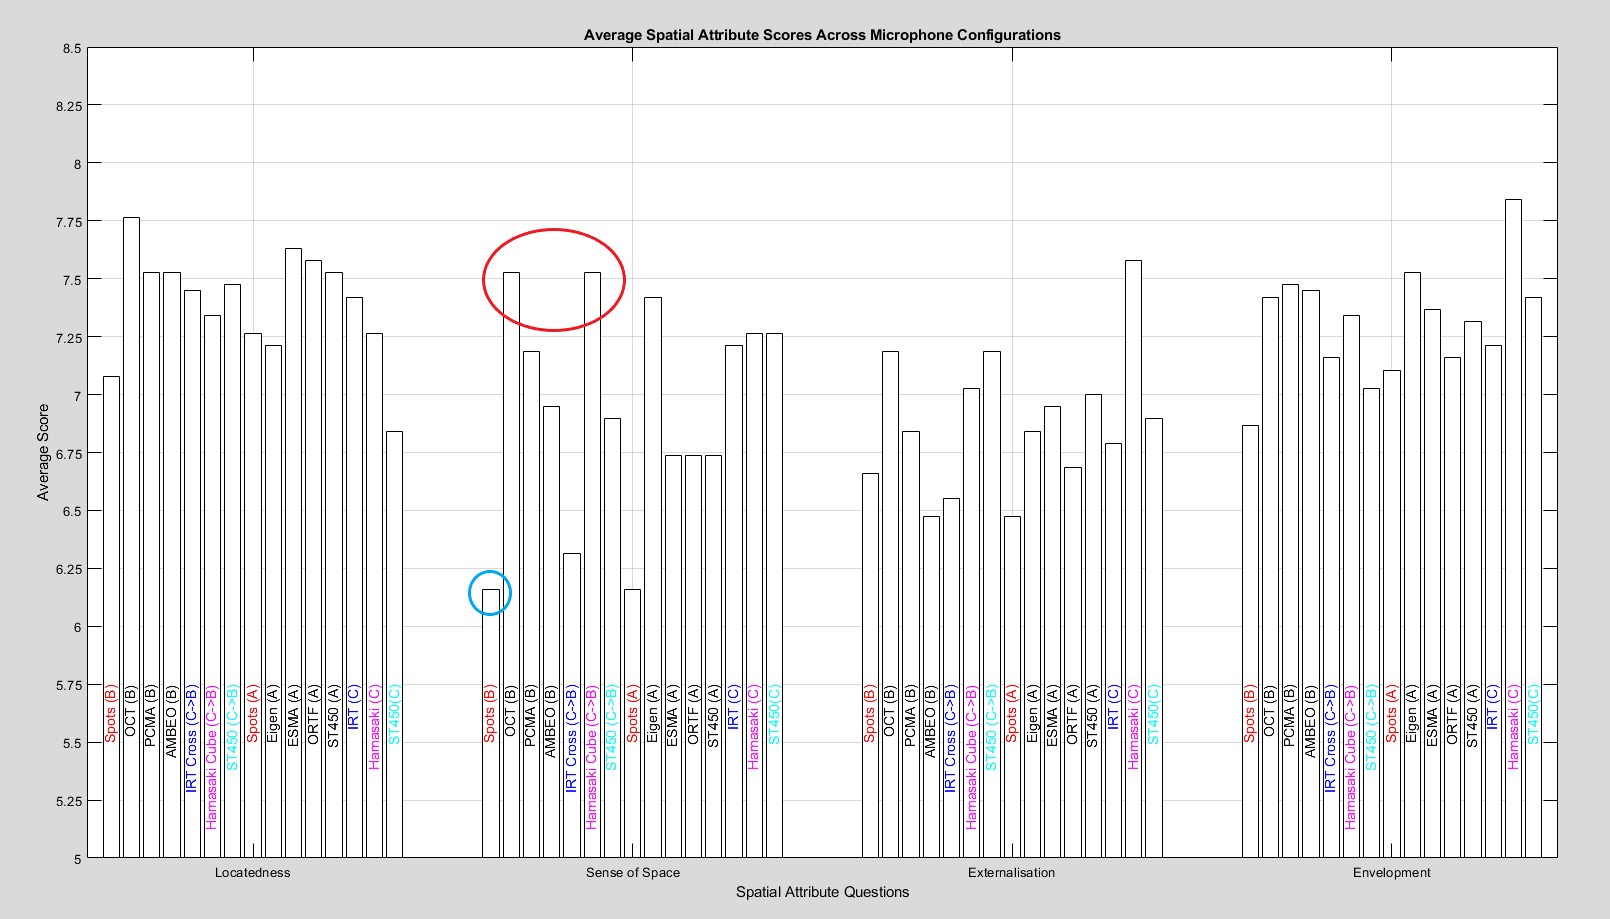
\includegraphics[width=0.5\textwidth]{images/plots/allMics_edit.PNG}
			\caption{Bar chart of the average SA score across all microphone configurations where (X) indicates the microphone location. The microphone names are displayed on their corresponding bar chart where (C->B) indicates a microphone from position C whilst viewing from B and (C) indicates a microphone from position C whilst viewing from position A}
			\label{image:sa_allmics} 
		\end{figure}


	






% =========----------	[ Space left here for distraction free mode] ----------==========%









\subsection{Analysis 3: What is the effect of using Directional or Diffuse-Field Arrays?}
	\label{ana3}

		Section~\ref{ana2} revealed no significant difference between using any of the different microphone arrays apart from when it comes to a 'Sense of Space'. However the difference was only found between using the spot mic mix against mixing the spot mics with either the OCT array or the Hamasaki Cube. As both of these microphone arrays belong to different groups (OCT is used as a directional array and the Hamasaki Cube as a diffuse field array) and were not significantly different from each other, it can also be stated that the use of directional or diffuse field arrays is also not statistically significant.

		Analysing the bar chart in figure~\ref{image:sa_allmics} however it is possible to come to some conclusions about particular microphone configurations. For example, looking at the scores for Sense of Space, the three diffuse field microphone in position C whilst viewing from position A can be said to objectively perform worse than the three of the directional microphones at position A (ESMA, ORTF, ST450). However as the Eigenmke scores higher than all of them, drawing a conclusion that one microphone type is superior would be a incorrect. A more collated visualisation of overall microphone configuration performance can be seen in figure~\ref{image:sa_allmic_avgQ}, highlighting the narrow lead of the OCT microphone configuration.

		\textbf{Conclusion}
		There appears to be no significant effect of using either a directional or diffuse-field microphone array providing that spot microphones alone are not used

		\begin{figure}
			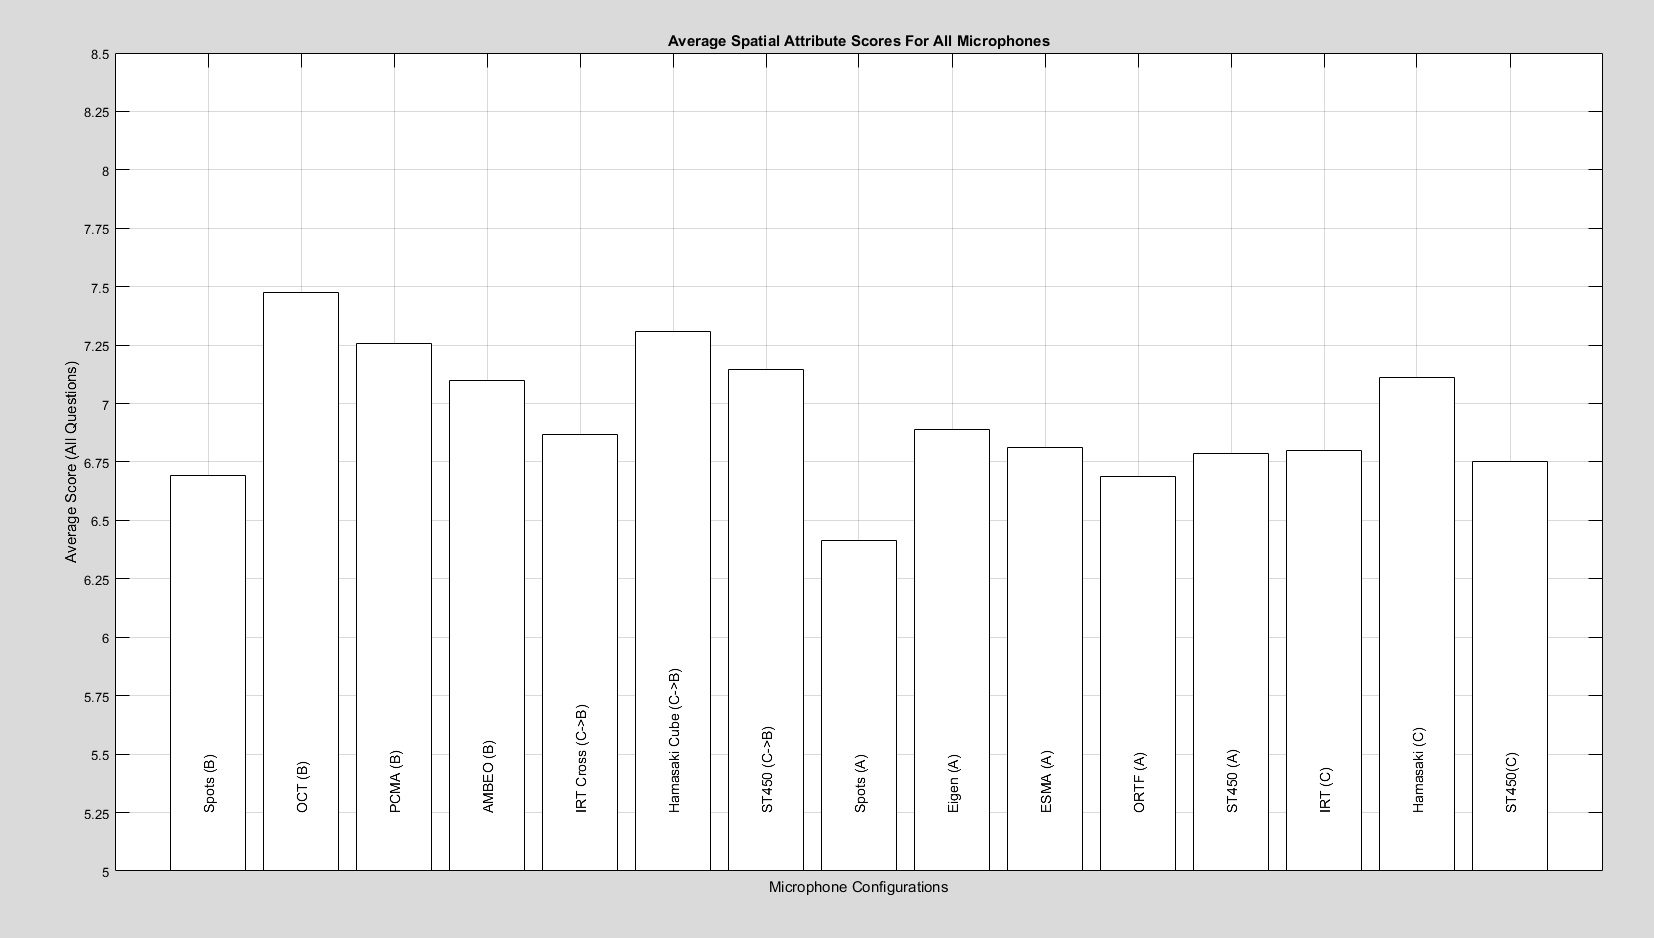
\includegraphics[width=0.5\textwidth]{{images/plots/ana3_allmics_performance.PNG}}
			\caption{}
			\label{image:sa_allmic_avgQ} 
		\end{figure}		
	






% =========----------	[ Space left here for distraction free mode] ----------==========%









\subsection{Analysis 4: Is there a difference in perception of timbre with difference viewing positions?}
\label{ana4}
		
	The effect of different viewing positions on participants perception of timbre can be assessed by comparing the data collected for microphones that were shared across both viewing positions which includes the spot microphones and microphone arrays from position C. Figure~\ref{image:ta_sharedmics} shows the percentage of participants that selected each timbral attribute for each microphone. Table~\ref{ana4:barData} presents the corresponding data showing the percentage difference between each microphone pair (each microphone at both positions) calculated by subtracting the results for microphones at position B from the same microphones at position A. For each timbral attribute, the average results column indicates whether the attribute was selected by more participants for viewing position A (positive number) or position B (negative number). By looking at the table it can be seen that across all microphones the timbral attributes 'Realistic' and 'Loud' share the trend that they were selected by an equal or greater percentage of participants for viewing position A. The timbral attribute 'Realistic' experienced the greatest variation between viewing positions with an average difference of 19\%. Though the increased frequency of participants selecting 'Loud' is only by a minor amount, it is possible that the consistency is caused simply by the fact that viewing position A is closer to the musicians thus increasing the possibility for participants to perceive the audio as 'Loud'. \\

	\begin{figure}
		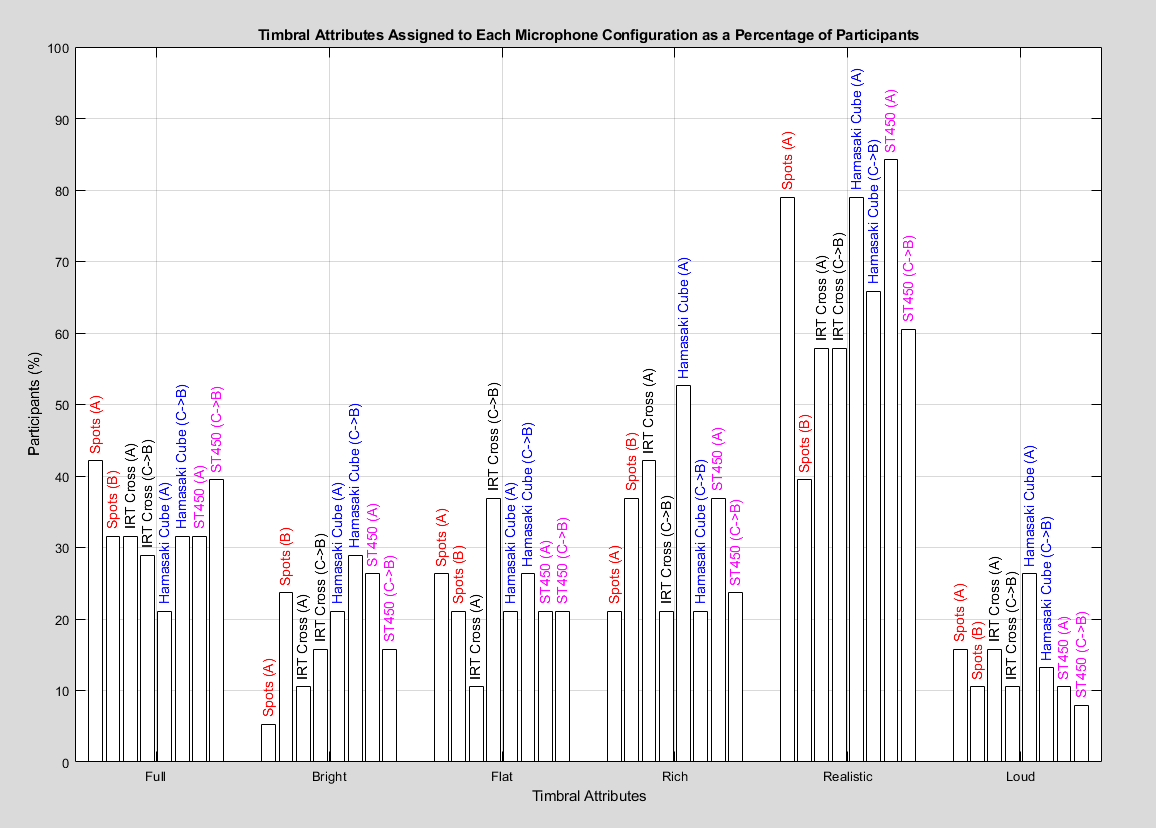
\includegraphics[width=\linewidth]{images/plots/bar_sharedMics.PNG}
		\caption{Bar chart showing the timbral attributes chosen for each microphone array shared between viewing position A and B as a percentage of participants}
		\label{image:ta_sharedmics} 
	\end{figure}	

	\begin{table}[h]
	\centering
	\resizebox{\linewidth}{!}{%
	\hspace{-15pt}
		\begin{tabular}{|>{\cen}m{15mm} |>{\cen}m{9.1mm} |>{\cen}m{9.5mm}| >{\cen}m{15mm}| *{2}{>{\cen}m{8mm}|}} \hline
		\multicolumn{1}{|>{\cen}m{12mm}|}{\multirow{2}{*}{Attributes}} & \multicolumn{4}{c|}{Microphones (\%)} & \multicolumn{1}{c|}{\multirow{2}{*}{\textbf{Averaged}}} \\ \cline{2-5}
		& Spots & IRT Cross & Hamasaki Cube & ST450 & \\ \hline
		Full & 10.53 & 2.63 & -10.53 & -7.89 & -1.32  \\ \hline
		Bright & -18.42 & -5.26 & -7.89 & 10.53 & -5.26 \\ \hline
		Flat & 5.26 & -26.32 & -5.26 & 0 & -6.58 \\\hline
		Rich & -15.79 & 21.05 & 31.59 & 13.16 & 12.5 \\ \hline
		Realistic & 39.47 & 0 & 13.16 & 23.68 & 19.08 \\ \hline
 		Loud & 5.2 & 5.2 & 13.16 & 2.63 & 6.58 \\ \hline
		\end{tabular}}
		\caption{Table showing the percentage difference between each pair of microphones calculated by $A - B$}
		\label{ana4:barData}
	\end{table}



	\textbf{Conclusion} \\

		In terms of timbre there appears to be little difference made by watching the performance from either position. The attributes effected most by changing viewing positions are a sense of whether things sounded realistic for which position A showed a preference. This increased difference however is mostly influenced by the large difference in spot microphone scores where there is a 39.5\% increase from the low 39.5\% of participants regarding the spot mics at position B to sound realistic to the 79\% of participants regarding the spot mics at position A to sound realistic. 

		It is hypothesised by the author that this is due to the unnatural lack of room acoustics heard when positioned at a distance where the sound of the room is expected to be heard. As the participant is standing much closer to the musicians at position A where the direct to reverb ratio is naturally much higher, the lack of room acoustics may be less noticeable and still be perceived as realistic. As a consequence of a lack of room acoustics present in the spot microphone mix, sound sources can be perceived more spatially isolated from one another. The unnaturalness of this is possibly less obvious when fully surrounded by the musicians as experienced at position A as this introduces an unnatural separation of the musicians for a listening experience. When viewing from position B however, as the musicians can be seen closer together, the unnatural sound source separation perceived may stand out to participants and further affect their judgement. \\


	% \begin{center}
	% \begin{table}
	% 	\begin{tabular}{r >{\centering\arraybackslash}p{30mm} c}
	% 		Attribute & Absolute Average Percentage Difference & Sway \\
	% 		Full & 7.89 & -1.32 \\
	% 		Bright & 10.53 & -5.26 \\
	% 		Flat & 9.21 & -6.58 \\
	% 		Rich & 20.39 & 12.5 \\
	% 		Realistic & 19.08 & 19.08 \\
	% 		Loud & 6.58 & 6.58 
	% 	\end{tabular}
	% 	\caption{Percentage difference}
	% 	\label{ana4:perDiff}
	% \end{table}
	% \end{center}
	






% =========----------	[ Space left here for distraction free mode] ----------==========%









\subsection{Analysis 5: Is there a correlation between spatial attribute score and selected timbral attributes?}

	Correlation coefficients were calculated for each combination of spatial attribute score against timbral attribute score. Most calculations returned weak correlations with $p > 0.05$ other than two timbral attributes specifically when comparing against the 'Envelopment' spatial attribute. Figure~\ref{image:corr_env} shows the line of best fit for all timbral attribute scores against the spatial attribute scores for 'Envelopment'. The dashed lines indicate a statistically significant correlation as found with the timbral attributes 'Full' and 'Realistic'. The graph indicates that there is a significant positive correlation between the increase in sense of 'Envelopment' in the virtual environment with the sense of the virtual environment sounding 'Realistic'.

	The data also indicates a negative correlation between participants sense of 'Envelopment' and their perception of the timbre sounding 'Full'. The reason as to why this is is not exactly clear. It could be said that participants perception of 'Full' may mean an unnatural abundance of bass frequencies which may sound unrealistic. If this is the case, as we can see from the positive correlation between a sense of 'Envelopment' and a sense of the environment sounding 'Realistic', that an unrealistic sounding environment would lead to a decrease in participants sense of 'Envelopment'. 

	\textbf{Conclusion}

	The only spatial attribute to show a significant correlation with timbral attribute data is 'Sense of Space' with a positive correlation for a perception of the mix sounding 'Realistic' and a negative correlation for the perception of the mix sounding 'Full'.

	\begin{figure}
		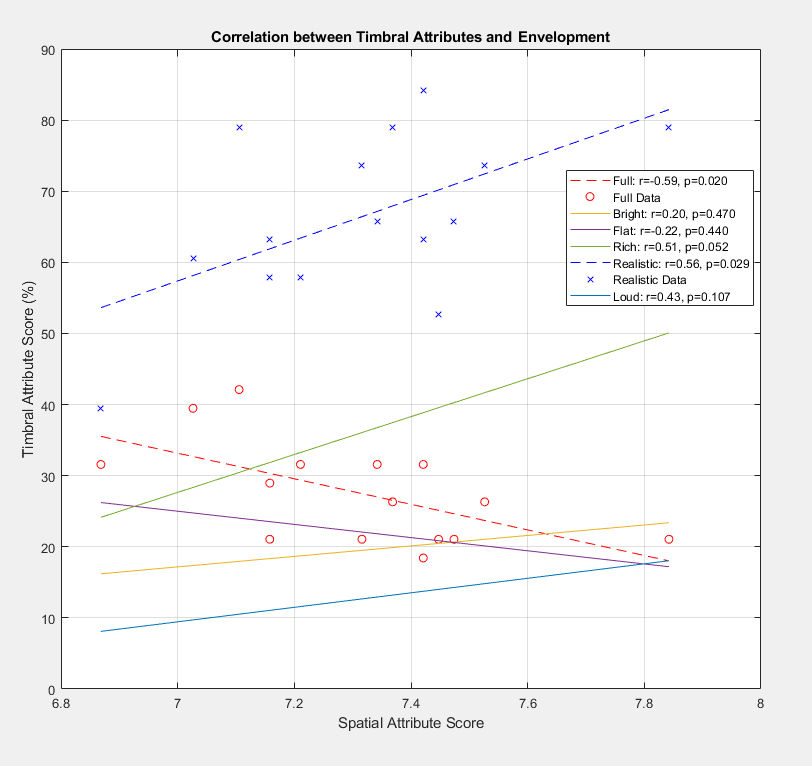
\includegraphics[width=\linewidth]{images/plots/sa_ta_corr_env.PNG}
		\caption{Graph showing correlations between Timbral Attribute and Envelopment scores where dashed lines indicate a statistically significant correlation for which their individual data points have also been plotted.}
		\label{image:corr_env} 
	\end{figure}		

	






% =========----------	[ Space left here for distraction free mode] ----------==========%









\subsection{Analysis 6: Enjoyment Factor}

	As VR is designed to entertain, participants were asked to rate on a scale of 1-10 how much they felt they enjoyed the experience. Figure~\ref{image:enjoyment} shows the line of best fit for everage enjoyment rating againt average spatial attribute for each microphone for both viewing position A and B.
	

	\begin{figure}
		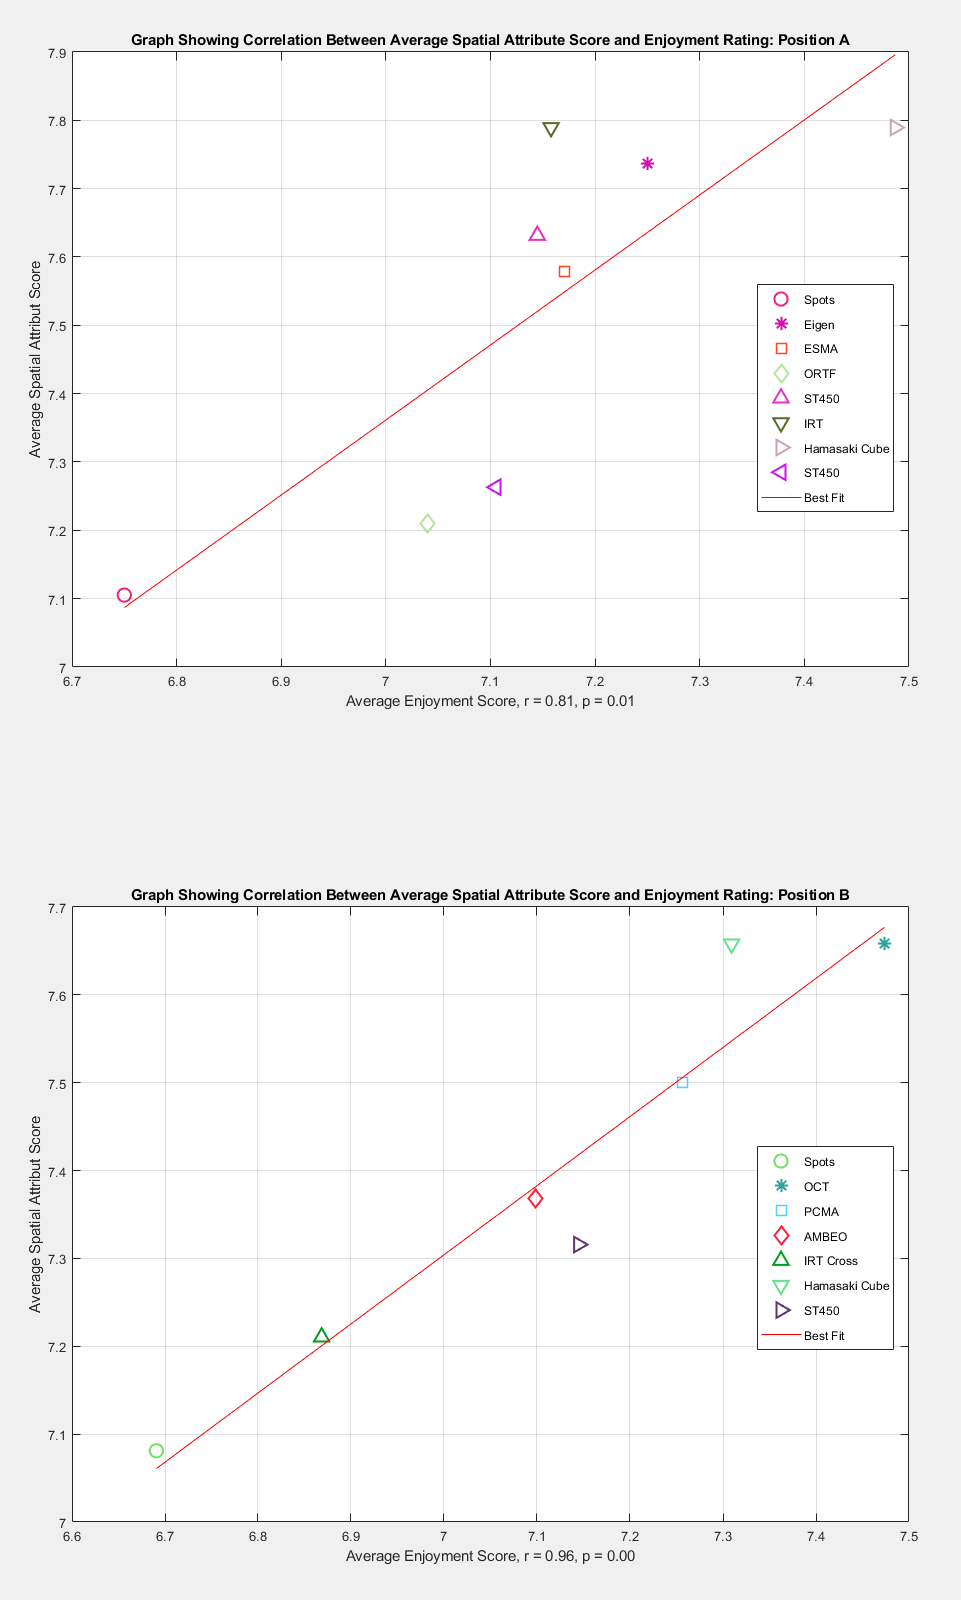
\includegraphics[width=0.5\textwidth]{images/plots/enjoyment_corr_V1.PNG}
		\caption{Two graphs showing a positive correlation between enjoyment rating and spatial attribute scores for viewing positions A (Top) and B (Bottom).}
		\label{image:enjoyment} 
	\end{figure}		


	\section{Analysis Summary}
		% Summarise the results

		The analysis of the data can be summarised as follows:\\

		Analysis 1: Viewing the performance from position A (360\textdegree~perspective) or position B (180\textdegree~perspective) does not significantly influence participants judgement on the proposed spatial attributes. \\

		Analysis 2: When compared to a spot microphone only mix, the OCT and Hamasaki Cube were found to be statistically significant with regards to the spatial attribute 'Sense of Space'. This can be seen as a significantly poor performance from the spot microphones at viewing position B. Though little statistical significance was found between the different microphone arrays, by analysing figure~\ref{image:sa_allmics} in section~\ref{ana2} we can determine which microphones are overall the best choice with regards to this listening test. The two microphone arrays that showed statistical significance, the OCT and Hamasaki Cube also happen to consistently be among the top scoring microphone arrays across all spatial attributes. \\

		Analysis 3: There appears to be no significant difference between using either a direct or diffuse-field microphone array so long as spot microphones alone are not used.\\

		Analysis 4: Timbre itself seems to be unaffected by the viewing positions. However participants perception of the mix sounding 'realistic' and 'loud' appears to be the most affected with a higher score for viewing position A. It is hypothesised that this is due to the unnatural room acoustic and sound source separation caused when listening to the spot mic mix that skews the result this way.\\

		Analysis 5: A statistically significant positive correlation was found between 'Sense of Space' and the perception of the mix being 'realistic'. A significant negative correlation was also found between 'Sense of Space' and the perception of the timbre sounding 'Full'.\\

